\section{Конструкторская часть}

\subsection{Требования к программному обеспечению}
Программное обеспечение состоит из драйвера, реализованного в виде
загружаемого модуля ядра, который посредством считывания и обрабатывания информации клавиш и стиков геймпада
реализует функционал обычной компьютерной мыши.

\subsection{Реализация драйвера}
В основе данного ПО лежит реализация исходного USB драйвера геймпада.
Его работа заключается в регистрации своего объекта драйвера с USB
подсистемой.

\subsection{Регистрация драйвера}
Для регистрации драйвера в системе имеется структура \textit{usb\_driver}.\textit{struct
usb\_driver} определена в /include/linux/usb.h. Данная структура представлена ниже на Рисунке \ref{USB-driver}. 

\begin{figure}[h!]
	\centering
	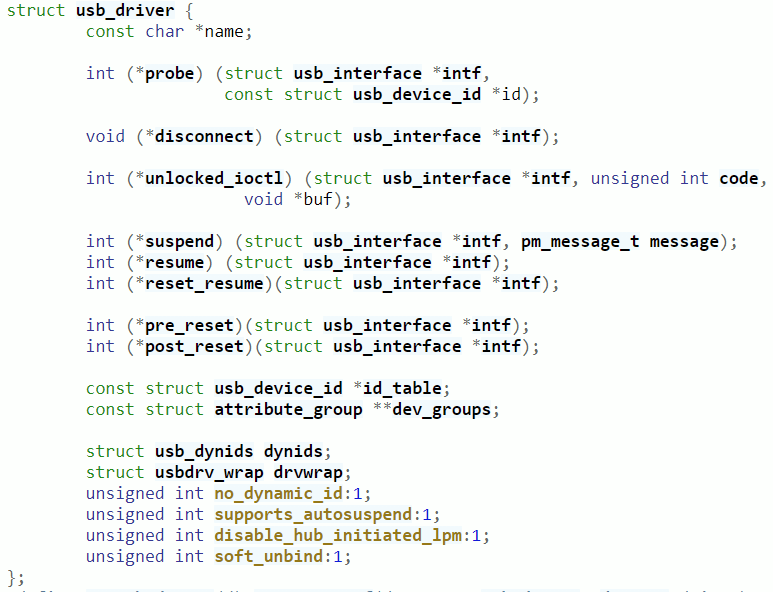
\includegraphics[scale=0.88]{img/usb-driver.png}
	\caption{Структура usb\_driver}
	\label{USB-driver}
\end{figure}\par

Для регистрации USB драйвера мыши следует рассматривать
следующие основные поля структуры:
\begin{itemize}
	\item \textit{name} --- имя драйвера. Оно должно быть уникальным и обычно совпадает с именем модуля;
	\item \textit{probe} --- указатель на функцию, которую подсистема USB ядра вызывает при подключении устройства;
	\item \textit{disconnect} - указатель на функцию, которую подсистема USB ядра вызывает при отключении
	устройства. Внутри указанной функции выполняется освобождение
	памяти и отмена регистрации устройства;
	\item \textit{id\_table} --- указатель на структуру\textit{ usb\_device\_id}, описывающую таблицу
	идентификаторов USB драйверов, необходимую для быстрого
	подключения устройств. В случае ее отсутствия, функция probe не
	сможет быть вызвана.
\end{itemize}\par
После инициализации структуры \textit{usb\_device\_id} выполняется вызов
макроса \textit{MODULE\_DEVICE\_TABLE}. При компиляции процесс извлекает
информацию из всех драйверов и инициализирует таблицу устройств. При
подключении устройства, ядро обращается к таблице, где выполняется поиск
записи, соответствующей идентификатору устройства. В случае нахождения
такой записи, выполняется инициализация и загрузка модуля.

\subsection{Подготовка к эмуляции событий мыши}
Чтобы пометить устройство, как способное генерировать определенные события, нужно 
применить функцию \textit{input\_set\_capability}. Данная функция определена в /include/linux/usb.h.
Ниже на Рисунке \ref{input_set} представлен её вид.
\begin{figure}[h!]
	\centering
	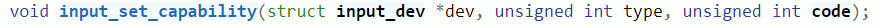
\includegraphics[scale=0.9]{img/input-set-capability.png}
	\caption{Сигнатура функции \textit{input\_set\_capability}}
	\label{input_set}
\end{figure}\par

Поля функции:
\begin{itemize}
	\item \textit{dev} --- устройство, способное передавать или принимать событие;
	\item \textit{type} --- тип события (EV\_KEY, EV\_REL, EV\_ABS, etc...);
	\item \textit{code} --- код события (в нашем случае это код нажимаемых клавиш и передвигаемых стиков геймпада).
\end{itemize}\par
% https://www.unix.com/man-page/suse/9/input_set_capability

Используемые в данной работе типы событий:
\begin{itemize}
	\item EV\_KEY используется для описания изменений состояния клавиатур,
	 кнопок или других устройств, похожих на клавиши. Этим событием описываются все нажатия кнопок геймпада;
	\item EV\_REL используется для описания изменений относительных значений оси, например, перемещения мыши.
	Этим событием описываются движения стика, при помощи которого курсор мыши должен изменять своё положение.
\end{itemize}\par

%https://www.kernel.org/doc/html/latest/input/event-codes.html

\subsection{Обработка сообщений от устройства}
Внутри драйвера реализована функция \textit{xpad\_irq\_in},
позволяющая обрабатывать сообщения, отправленные устройством.
\begin{figure}[h!]
	\centering
	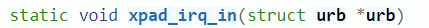
\includegraphics[scale=1]{img/xpad-irq-in.png}
\end{figure}\par
Внутри данной функции происходит обработка нажатых на геймпаде клавиш, а также движений стиков.
Для того, чтобы сообщить о новом событии нажатия кнопки,изменения положения использцется функция \textit{do\_action}.
Ниже на Рисунке \ref{input_report} приведён её вид.

\begin{figure}[h!]
	\centering
	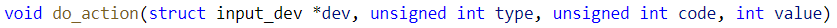
\includegraphics[scale=0.9]{img/action-naming.png}
	\caption{Функция \textit{do\_action}}
	\label{input_report}
\end{figure}\par
\newpage

Рассмотрим её поля поподробнее:
\begin{itemize}
	\item \textit{dev} --- устройство, сгенерировавшее событие;
	\item \textit{type} --- тип события;
	\item \textit{code} --- код события;
	\item \textit{value} --- значение события.
\end{itemize}\par
%/include/linux/input.h

\subsection{Схемы алгоритмов работы драйвера}
Ниже на Рисунках \ref{driver-work1} и \ref{driver-work2} представлена схема алгоритма работы драйвера геймпада.

\begin{figure}[h!]
	\centering
	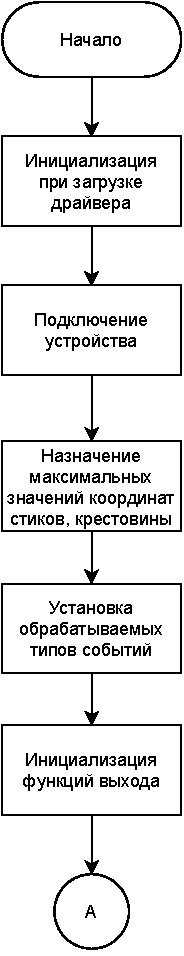
\includegraphics[scale=1.5]{img/driver-work1.pdf}
	\caption{Схема алгоритма работы драйвера геймпада}
	\label{driver-work1}
\end{figure}
\newpage

\begin{figure}[h!]
	\centering
	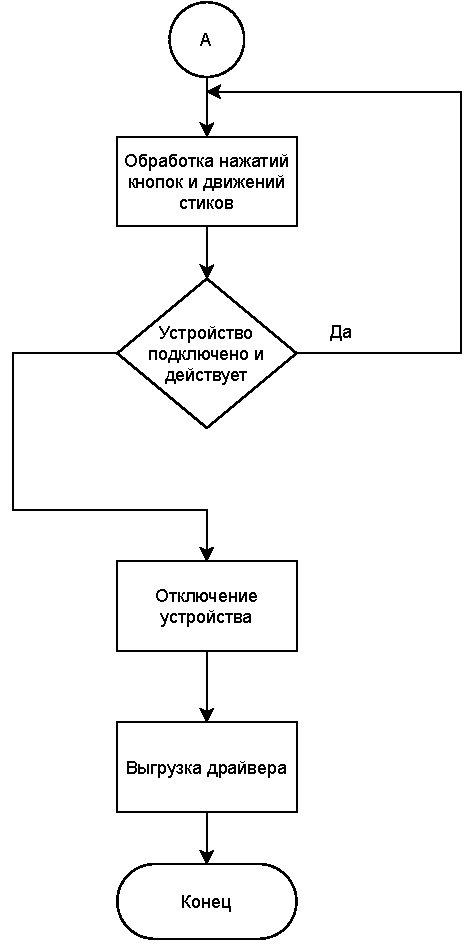
\includegraphics[scale=1.5]{img/driver-work2.pdf}
	\caption{Схема алгоритма работы драйвера геймпада}
	\label{driver-work2}
\end{figure}

\pagebreak